\documentclass{article}
\usepackage[normalem]{ulem}
\usepackage[12pt]{extsizes}
\usepackage[utf8]{inputenc}
\usepackage[T2A]{fontenc}
\usepackage{amsmath}
\usepackage{amssymb}
\usepackage{mathtools}
\usepackage{hyperref}
\usepackage{amsfonts}
\usepackage{cmap}
\usepackage{multicol}
\usepackage{comment}
\usepackage[parfill]{parskip}

\usepackage{listings}
\usepackage{color}
\usepackage{colortbl}
\usepackage{xcolor}
\usepackage[left=1.5cm,right=2cm,top=2cm,bottom=2cm,bindingoffset=0.1cm]{geometry}
\usepackage[russian]{babel}
\usepackage[pdf]{graphviz}
\usepackage{tikz}
\usepackage{pgfplots}
\usepgfplotslibrary{polar}
\usepackage{etoolbox} % <--- added
\AtBeginEnvironment{enumerate}{\linespread{.84}\selectfont}
\newcommand{\ctd}{\begin{flushright} $\square$ \end{flushright}}
%%% Работа с картинками
\usepackage{graphicx}  % Для вставки рисунков
  % папки с картинками
\setlength\fboxsep{3pt} % Отступ рамки \fbox{} от рисунка
\setlength\fboxrule{1pt} % Толщина линий рамки \fbox{}
\pagenumbering{gobble}

\hypersetup{
    colorlinks=true,
    linkcolor=black,
    filecolor=magenta,      
    urlcolor=blue,
    pdftitle={Calculus},
    pdfpagemode=FullScreen,
    }
\lstset{ %
  language=C++, % the language of the code
  basicstyle=\footnotesize\ttfamily, % the size of the fonts that are used for the code
  numbers=left, % where to put the line-numbers
  numberstyle=\footnotesize\color{black},  % the style that is used for the line-numbers
  stepnumber=0, % the step between two line-numbers. If it's 1, each line 
       % will be numbered
  numbersep=0.7em,       % how far the line-numbers are from the code
  backgroundcolor=\color{white!95!gray}, % choose the background color. You must add \usepackage{color}
  showspaces=false,      % show spaces adding particular underscores
  showstringspaces=false,% underline spaces within strings
  showtabs=false,        % show tabs within strings adding particular underscores
  frame=single, % adds a frame around the code
  rulecolor=\color{black},        % if not set, the frame-color may be changed on line-breaks within not-black text (e.g. commens (green here))
  tabsize=2,    % sets default tabsize to 2 spaces
  %captionpos=b,% sets the caption-position to bottom
  breaklines=true,       % sets automatic line breaking
  breakatwhitespace=false,        % sets if automatic breaks should only happen at whitespace
  %title=\lstname,       % show the filename of files included with \lstinputlisting;
       % also try caption instead of title
  identifierstyle=\color{black!50!green},  
  keywordstyle=\color{blue},      % keyword style
  commentstyle=\color{gray},      % comment style
  stringstyle=\color{purple},      % string literal style
  escapeinside={\%*}{*)},% if you want to add a comment within your code
  morekeywords={n,k},    % if you want to add more keywords to the set
  morecomment=[l][\color{black!50!green}]{\#}, % to color #include<cstdio> 
  morecomment=[s][\color{gray!50!black}]{/**}{*/}
}

\usepackage{amsmath,amssymb}
\usepackage{ stmaryrd }
\usepackage{ dsfont }
\usepackage{subfiles}

\newcommand{\updownarrows}{\mathbin\uparrow\hspace{-.5em}\downarrow}
\newcommand{\downuparrows}{\mathbin\downarrow\hspace{-.5em}\uparrow}
\newcommand{\defeq}{\stackrel{\mathclap{\normalfont\mbox{def}}}{=}}
\newcommand{\defLeftrightarrow}{\xLeftrightarrow{def}}

\usepackage{fancyhdr}
\pagestyle{fancy}
\fancyhf{}

\fancyhead[C]{Математический анализ} % Центральный заголовок
\fancyhead[L]{КТ ИТМО - 2 Семестр}
\fancyhead[R]{Кохась Константин}


\usepackage{tocloft}

\renewcommand{\cftsecfont}{\normalfont}
\renewcommand{\cftsecpagefont}{\normalfont}
\renewcommand{\cftsubsecfont}{\normalfont}
\renewcommand{\cftsubsecpagefont}{\normalfont}


\setlength{\cftsecindent}{0em}
\setlength{\cftsubsecindent}{0em}
\cftsetpnumwidth{0em}
\cftsetrmarg{0em}

% Разные определения
\newcommand{\abs}[1]{\left|{#1}\right|}
\newcommand{\norm}[1]{\lVert{#1}\rVert}
\newcommand{\stk}[2]{\stackrel{\eqref{#1}}{#2}}
\newcommand{\D}{\Delta}
\newcommand{\pderiv}[2]{\frac{\partial #1}{\partial #2}}
\newcommand{\appr}[1]{\xrightarrow[#1]{}}
\newcommand{\scal}[1]{\left\langle #1 \right\rangle}
\newcommand{\F}{\mathcal{F}}


% Числовые множества
\newcommand{\Var}{\text{Var}}
\newcommand{\R}{\mathbb{R}}
\renewcommand{\C}{\mathbb{C}}
\newcommand{\N}{\mathbb{N}}
\newcommand{\Q}{\mathbb{Q}}
\newcommand{\Z}{\mathbb{Z}}


% Необходимость, достаточность
\newcommand{\nec}{{$\Rightarrow$}}
\newcommand{\suff}{{$\Leftarrow$}}


% Буквенные \Re и \Im
\DeclareMathOperator{\@custom@Re}{Re}
\DeclareMathOperator{\@custom@Im}{Im}
\renewcommand{\Re}{\@custom@Re}
\renewcommand{\Im}{\@custom@Im}

% Еще переопределения
\renewcommand{\emptyset}{\varnothing}

% Математические операторы
\DeclareMathOperator{\rank}{rank}
\DeclareMathOperator{\mes}{mes}
\DeclareMathOperator{\diam}{diam}
\DeclareMathOperator{\fix}{fix}
\DeclareMathOperator{\sgn}{sgn}
\DeclareMathOperator{\sign}{sgn}
\DeclareMathOperator{\vp}{v.p.}
\DeclareMathOperator{\Arg}{Arg}
\DeclareMathOperator{\Ln}{Ln}
\DeclareMathOperator{\Arcsin}{Arcsin}
\DeclareMathOperator{\Arccos}{Arccos}
\DeclareMathOperator{\Arctg}{Arctg}
\DeclareMathOperator{\Arcctg}{Arcctg}
\DeclareMathOperator{\Arsh}{Arsh}
\DeclareMathOperator{\Arch}{Arch}
\DeclareMathOperator{\Arth}{Arth}
\DeclareMathOperator{\Arcth}{Arcth}

\usepackage{dsfont}
\newcommand{\zero}{\mathds{O}}
\renewcommand{\ker}{\mathcal{K}er}
\newcommand{\rg}{rg}
\renewcommand{\span}{span}

% Интегралы до бесконечности
\newcommand{\iinf}[1]{\int\limits_{#1}^{+\infty}}
\newcommand{\ioinf}{\int\limits_{0}^{+\infty}}
\newcommand{\ipminf}{\int\limits_{-\infty}^{+\infty}}
\newcommand{\dint}{\displaystyle \int}
\newcommand{\integral}[2]{\displaystyle\int\limits_{#1}^{#2}}
\newcommand{\Segm}{\text{Segm}}


\newcommand{\deff}[1]{\underline{\textbf{#1}}}
\newcommand{\thmm}[1]{\underline{\textbf{#1}}}
\newcommand*\xor{\mathbin{\oplus}}
\newcommand{\mytilde}{\raisebox{0.5ex}{\texttildelow}}

\title{Математический Анализ. Теор Опрос}
\author{Чепелин Вячеслав}
\date{}

\begin{document}

\maketitle
\tableofcontents
\newpage

\section{Определения}

\subsection{Первообразная, неопределенный интеграл}

 \deff{def:} $f: \langle a,b\rangle \rightarrow \mathbb{R}$. $F$ называется \deff{первообразной} функции $f$, если:

\begin{enumerate}
    \item $F$ дифференцируема на $\langle a,b\rangle$.

    \item $\forall x \in \langle a,b\rangle: F'(x) = f(x) $.
\end{enumerate}

\deff{Неопределенный интеграл} $f$ --- это множество всех первообразных $f$.

\subsection{Теорема о существовании первообразной}

$f$ - непрерывна на $\langle a,b \rangle$. Тогда $f$ имеет первообразную на $\langle a,b\rangle$.

\subsection{Таблица первообразных}

Она переписывается из таблицы производных, просто в обратную сторону. Но есть две \uline{\emph{загадочные}} формулы:
     $$\displaystyle \int \cfrac{dx}{1-x^2} = \frac{1}{2}\ln \left|\cfrac{1+x}{1-x}\right| + C \quad \quad \int \cfrac{dx}{\sqrt{1+x^2}} = \ln \left|x + \sqrt{1+x^2}\right| + C$$

\subsection{Площадь, аддитивность площади, ослабленная аддитивность}

\deff{def:} \deff{Фигура} - это ограниченное подмножество в $R^2$. $\varepsilon$ - множество всех возможных фигур.

$\sigma: \varepsilon \rightarrow [0,+\infty)$ ---  назовем \deff{площадью}, если:
\begin{enumerate}
    \item Аддитивно: $A_1,A_2 \in \varepsilon, A_1\cap A_2 = \emptyset, \sigma(A_1\cup A_2) = \sigma(A_1)+\sigma(A_2)$
\item Нормировка: $\sigma ([a,b]\times[c,d]) = (b-a)(d-c)$.
\end{enumerate}


\deff{def:}  $\sigma:\varepsilon\rightarrow [0,+\infty)$ --- \deff{ослабленная площадь}, если выполнено:
\begin{enumerate}
    \item монотонна.
    \item нормирована.
    \item ослабленная аддитивность: Есть $E \in \varepsilon: l $ - вертик. прямая $L^-$ - левая полуплоскость, $L^{+}$ - правая полуплоскость (замкнутая полуплоскость), тогда  $E_1 = E\cap L^-, E_2 = E \cap L^+: \sigma(E)=\sigma(E_1)+\sigma(E_2)$
\end{enumerate}

\subsection{Определенный интеграл}

\deff{def:} $f: [a,b] \rightarrow \mathbb{R}$, $f$ - непр., $\sigma $- осл. адд площадь, тогда \deff{определенный интегралом} $f$ по отрезку $[a,b]$ назовем: $$\dint\limits_{a}^b f =\dint\limits_{a}^b f(x) dx =\sigma(\text{ПГ($f^+$,$[a,b]$)})-\sigma(\text{ПГ($f^-$,$[a,b]$)})$$

\subsection{Выпуклая функция}

 $f:\langle a,b\rangle\rightarrow \mathbb{R}$ --- \deff{выпукла} на промежутке $\langle a,b\rangle$, если:
$$\forall x_1,x_2 \in \langle a,b \rangle: \forall \alpha \in[0,1]:f(\alpha x_1+(1-\alpha)x_2)\leq \alpha f(x_1) + (1-\alpha) f(x_2)$$

\subsection{Выпуклое множество в $R^m$}

Множество $A \subset R^m$ \deff{выпукло}, если:
$$\forall x,y \in A , [x,y]\subset A: [x,y] = \{x+t(y-x), t\in[0,1]\} = \{(1-t)x + ty, t\in[0,1]\}$$

\subsection{Надграфик}

\deff{Надграфик} ($f$, $\langle c,d \rangle) = \{(x,y): x\in \langle c,d \rangle, y \geq f(x)  \}$

\subsection{Опорная прямая}

\deff{def:} Дано множество $A$ выпуклое в $R^2$. Прямая $L$ называется \deff{опорной} к $A$ в точке $x_0$, если $L$ проходит через $x_0$ и множество $A$ лежит в одной полуплоскости (замкнутой).

\subsection{Функция промежутка, аддитивная функция промежутка}

$\Segm ([a,b])$ - множество всевозможных отрезков, лежащих в $[a,b]$

$\varPhi: \Segm([a,b]) \rightarrow \mathbb{R}$ - \deff{функция для промежутка}.

Введем \deff{аддитивные функции для промежутка}:
$$\forall [p,q] \in \Segm[a,b]: \forall c \in (p,q): \varPhi([p,c]) + \varPhi(c,q)= \varPhi([p,q])$$




\subsection{Плотность аддитивной функции промежутка}

\deff{def:} $f: \langle a,b \rangle \rightarrow \mathbb{R}$, $\varPhi: \Segm(\langle a,b \rangle) \rightarrow \mathbb{R}$ - а.ф.п:

$f$ - \deff{плотность} $\varPhi$: $\forall \Delta \in \Segm (\langle a,b\rangle):$$inf_{\Delta} f \cdot len(\Delta)\leq \varPhi(\Delta)\leq sup_{\Delta} f \cdot len(\Delta)$

\subsection{Кусочно-непрерывная функция, интеграл от неё}

\deff{def:} $f:[a.b] \rightarrow \mathbb{R}$ \deff{кусочно-непрерывной}, если:

$\exists A \ = \{x_1,\ldots,x_n\} \subset [a,b]$. Такая функция будет непрерывны на $[a,b]$, кроме этих точек, а в них происходят скачки.

$f$ - кусочно-непрерывно на $[a,b]$. $x_0 = a, x_n = b$. Положим $\integral{a}{b} = \sum\limits_{i=1}^{n+1}\integral{x_{i-1}}{x_i}f\Big|_{[x_{i-1},x_i]}$

\subsection{Почти первообразная}

\deff{def:} $F:[a,b] \rightarrow \mathbb{R}$ - \deff{почти первообразная} функции f, если:

$F$ - непр и $\exists A = \{x_1,\ldots,x_n\} \subset[a,b]$.
$\forall x \in [a,b] \textbackslash A: \exists F'(x) = f(x)$ и $\forall x \in A: \exists F'_+(x),F'_-(x)$

\subsection{Гладкий путь, вектор скорости, носитель пути}


Путь - $\gamma :[a,b] \rightarrow \mathbb{R}^m$. То есть $t\rightarrow (\gamma_1(t),\gamma_2(t),\ldots,\gamma_m(t)) = \gamma(t)$. Мы обычно думаем, что они непрерывны и дифференцируемы --- \deff{гладкие пути}.


$\gamma'(t) = (\gamma_1'(t),\gamma_2'(t),\ldots,\gamma_m'(t))$ - \deff{вектор скорости}.

\deff{Носитель пути} - траектория пути.

\subsection{Длина гладкого пути}

\deff{def:} Функция $l$, заданная на множестве гладких путей (непрерывны, дифференцируемы) называется длиной пути, если выполняются следующие условия:

\begin{enumerate}
    \item $l\geq 0$
    \item аддитивна: $\forall [a,b]$, $\forall \gamma:[a,b]\rightarrow\mathbb{R}^m$ для любого $c\in [a,b]: l(\gamma) = l(\gamma\Big|_{[a,c]}) + l(\gamma\Big|_{[c,b]})$
    \item $\gamma, \overline{\gamma}$ --- два пути. $C_{\gamma},C_{\overline{\gamma}}$ --- носители пути.
    
    Если $\exists T: C_{\gamma} \rightarrow C_{\overline{\gamma}}$ --- сжатие ($\forall M,N:\rho(T(M), T(N))\leq \rho(M,N)$), то $l(\overline{\gamma})\leq l(\gamma)$
    \item $\gamma$ - линейный путь, то $l(\gamma) = \rho(A,B)$, где $A$ - начало, $B$ - конец.
\end{enumerate}

Примеры ниже

\subsection{Вариация функции на промежутке}

\deff{def:} Пусть $f$ - любая из $[a,b] \rightarrow \mathbb{R}$. Тогда \deff{вариация функции} на $[a,b]$: 
$$\Var_a^b f = \sup (\sum\limits_{k=1}^n |f(t_k)-f(t_{k-1})|)$$
где $\tau = \{t_0,\ldots, t_n\}$ --- дробление отрезка

\subsection{Теорема о функциях ограниченной вариации}

Если для $f$ выполнено: $\Var_a^b f < + \infty$, то она называется \deff{ограниченной} вариации.

Я не знаю что тут надо

\subsection{Верхний и нижний пределы}


\deff{def:} $x_n$ - вещ. последовательность. Рассмотрим $y_n = \sup (x_n, x_{n+1},\ldots),z_n = \inf(x_n,x_{n+1},\ldots)$. $y_n$ - \deff{верхне огибающая}, $z_n$ - \deff{нижне огибающая}. 

$y_n$ - не возрастает, $z_n$ - не убывает. $\forall n: z_n\leq x_n \leq y_n$

Если изменить конечное число членов последовательности, то $y_n,z_n$ изменятся конечное число раз.

\deff{Верхний предел последовательности}--- $\overline{\lim\limits_{n\rightarrow \infty}}x_n=\lim y_n \in \overline{R}$

\deff{Нижний предел последовательности}--- $\underline{\lim\limits_{n\rightarrow \infty}}x_n=\lim z_n \in \overline{R}$


\subsection{Частичный предел}

\deff{def:} $(x_n)$ - вещ. последовательность $L\in \mathbb{R}$ - \deff{частичный предел} $x_n: \exists (n_k):n_1<n_2<\ldots: \lim\limits_{n\rightarrow \infty} x_{n_k}=L$.

\subsection{Вычисление длины пути в полярных координатах и длины графика}

\textbf{Примеры:}
\begin{enumerate}
    \item В $\mathbb{R}^2:\gamma(t) = (x(t),y(t))$ - обычные декартовы.

    $$l = \integral{a}{b}\sqrt{x'(t)^2+y'(t)^2} dt$$
    \item $\mathbb{R}^2$, полярные координаты $r(t)$,$\varphi(t)$
    $$l = \integral{a}{b} \sqrt{((r(t) \cos \varphi(t))')^2+((r(t) \sin\varphi(t))')^2} = \integral{a}{b} \sqrt{r(t)^2+r'(t)^2}dt$$
    \item Длина графика $x(t) =t, y(t) = f(t)$. 
    $$l = \integral{a}{b}\sqrt{1 + y'(x)^2}dx$$
\end{enumerate}


\subsection{Дробление отрезка, ранг дробления, оснащение, интегральная сумма Римана}

\deff{def:} $[a,b]$ \deff{дробление} отрезка $[a,b]$ (на $n$ частей):

$x_0 = a <x_1<x_2<\ldots <x_n=b$.

\deff{Ранг} дробления(мелкость) - $\max |x_k-x_{k-1}|$

\deff{Оснащение дробления} - $\{\xi_1,\ldots, \xi_n\}: \xi_i \in [x_{i-1},x_i]$

Пусть задана $f:[a,b] \rightarrow \R$. Тогда \deff{Риманова сумма}: $\sum\limits_{i=1}^n f(\xi_i)(x_i-x_{i-1})$.


\subsection{Кривая Пеано}

\deff{Кривая Пеано} - это путь в $\R^2$, такой, что я сначала разбиваю отрезок $[0,1]$ на 4 равных части так, что отображение первой части отрезка находится в части 1(см рисунок), второй части отрезка в части 2 и так далее. Потом повторяю то же самое в каждом квадратике. Потом повторяю то же самое в каждом квадратике квадратика и так далее. Изображение внизу описывает это построение поэтапно.

\begin{center}
   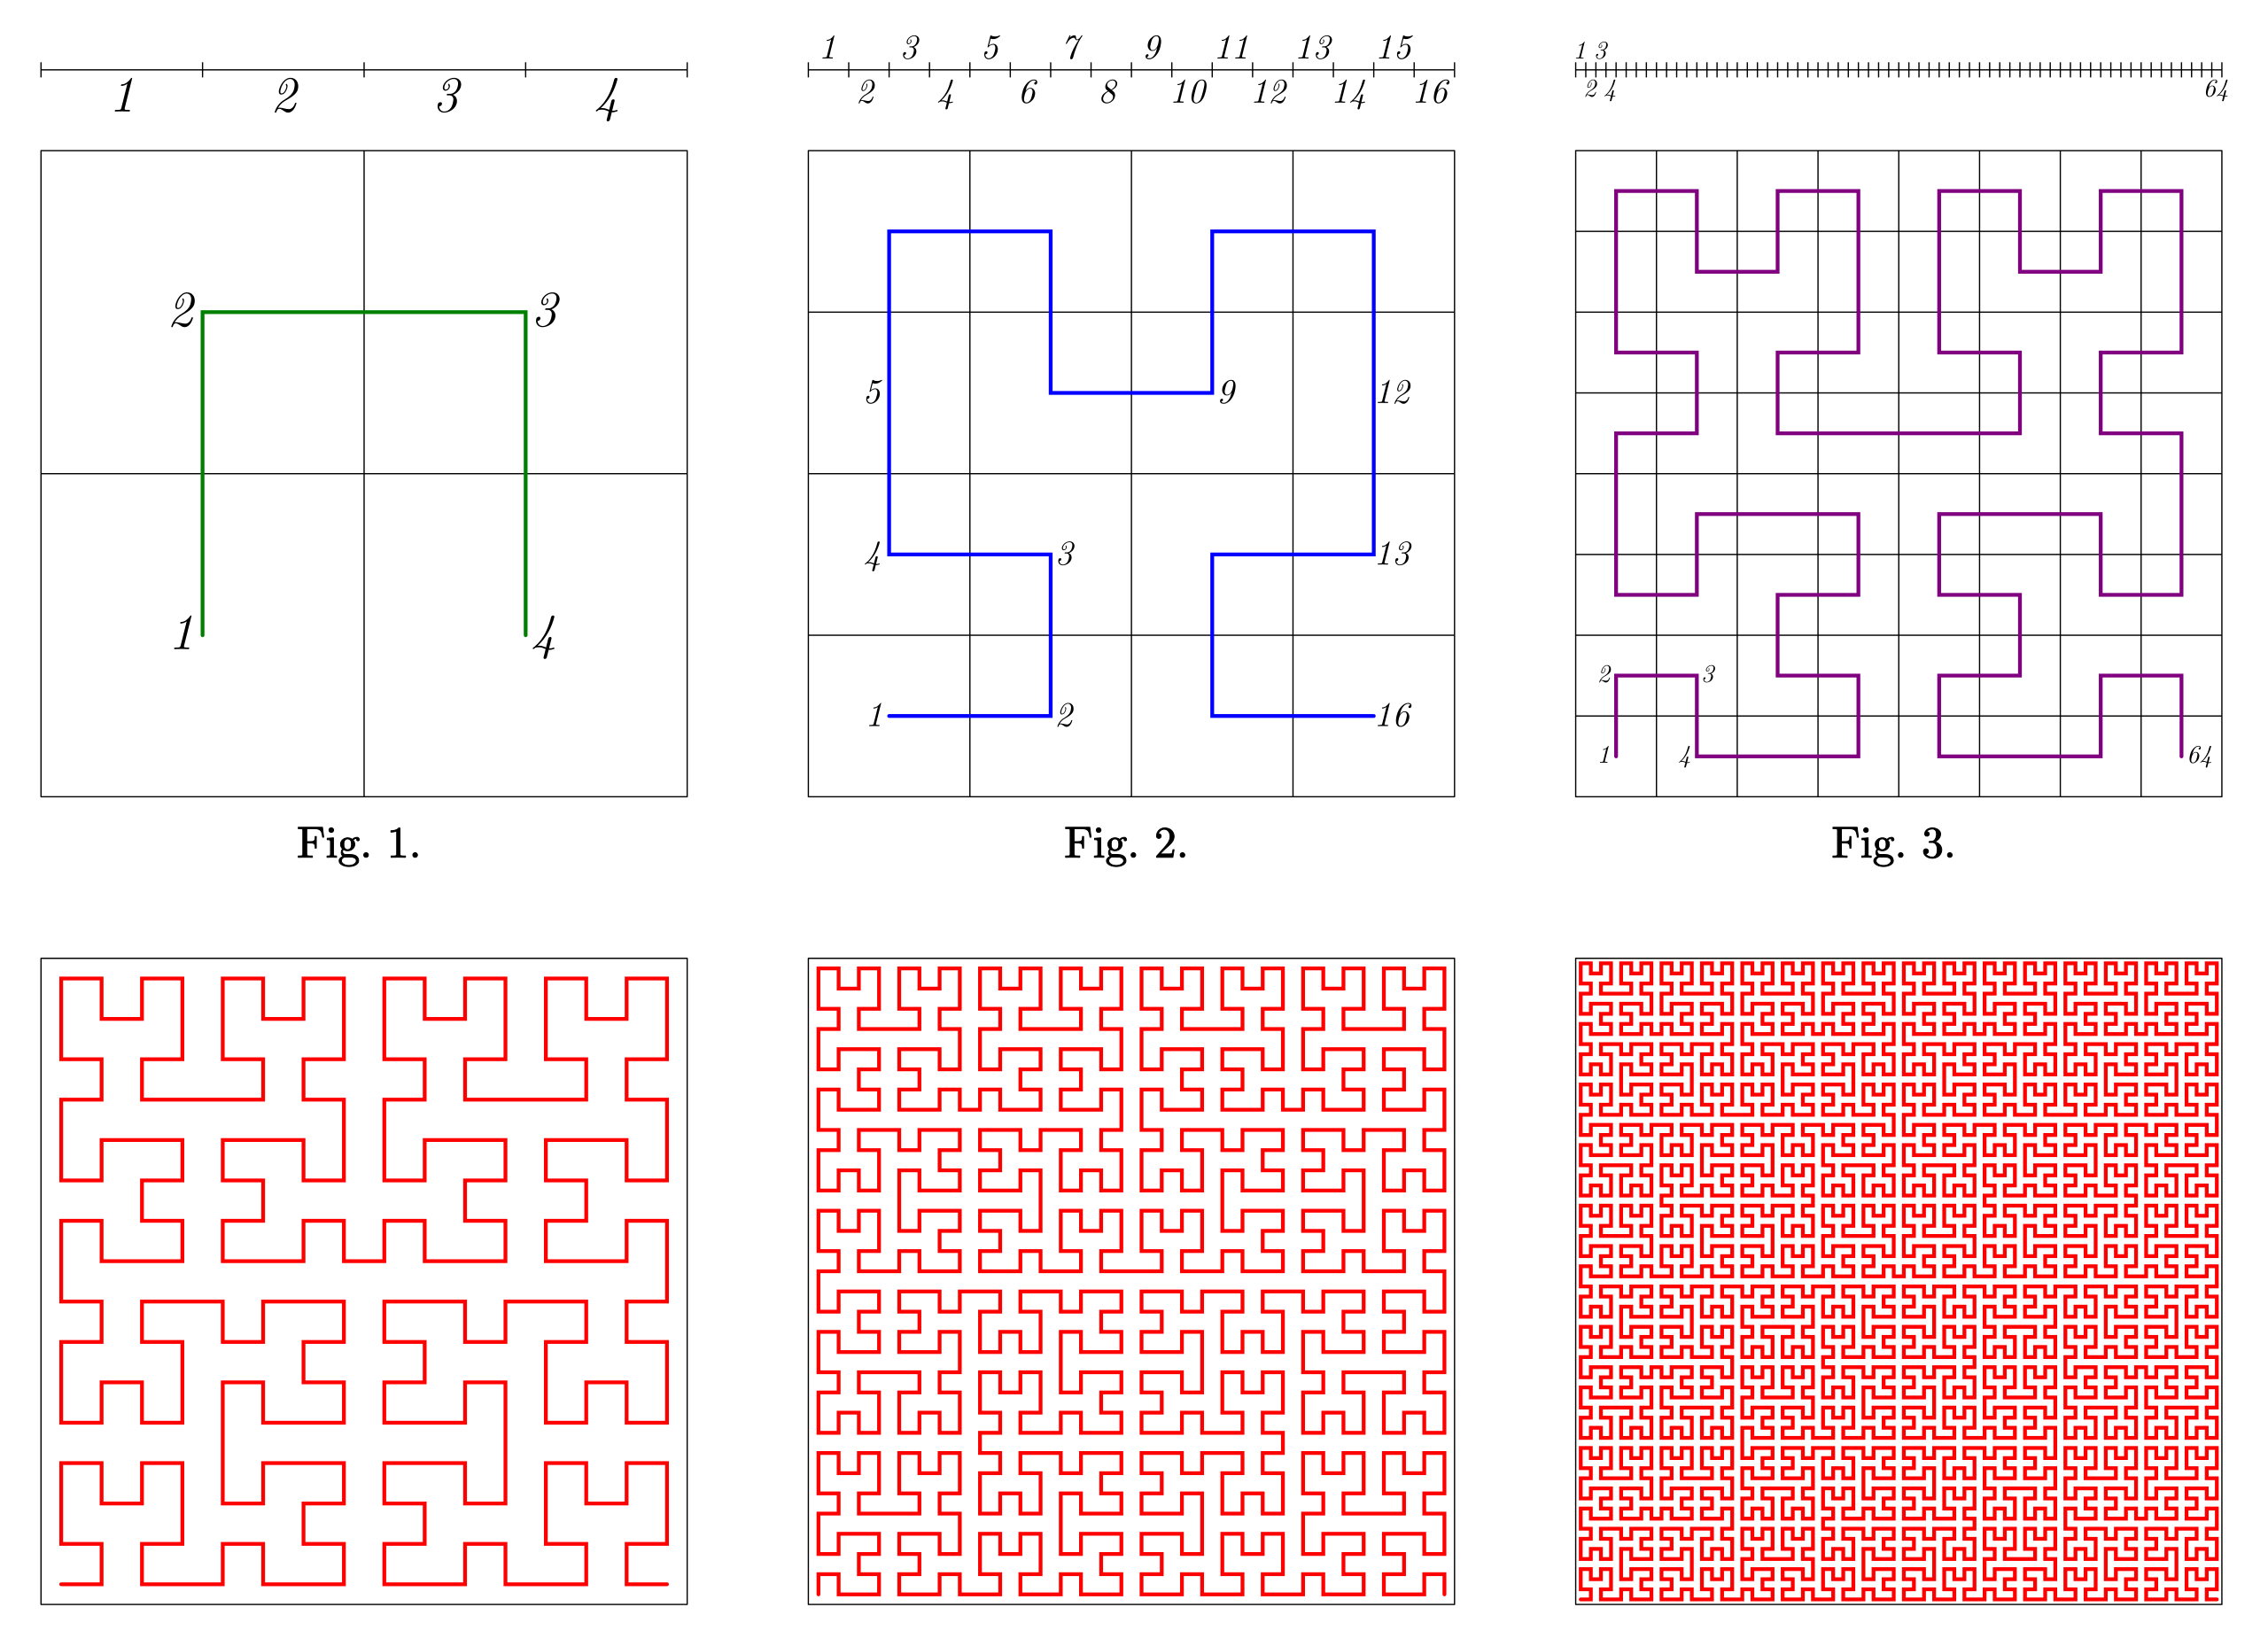
\includegraphics[width = 15 cm]{assets/integral_hilbert_curve.svg.png}
\end{center}

\subsection{Постоянная Эйлера}

$1+\cfrac{1}{2}+\cfrac{1}{3}+\ldots +\cfrac{1}{n}= \ln n + \gamma + o(1)$. Причем $\gamma \in [\cfrac{1}{2},\cfrac{5}{8}]$ - \deff{Постоянная Эйлера}

\subsection{Несобственный интеграл, сходимость, расходимость}

\deff{def:} $\varPhi(A):= \integral{a}{A}f(x) dx$

Если $\exists \lim\limits_{A \rightarrow b -0} \varPhi(A) \in \overline{R}$ - этот предел называется \deff{несобственным интегралом}

Если этот предел конечен, то говорят, что несобственный интеграл сходится, иначе - расходится.

\subsection{Критерий Больцано-Коши сходимости несобственного интеграла}

\textbf{Критерий Больцана-Коши} (сходимости несобственного интеграла):
  
  $\integral{a}{b}f(x)dx$ --- сходящаяся $\Leftrightarrow \forall \varepsilon >0:\exists \Delta \in (a,b): \forall A,B\in (a,b),  |\integral{A}{B}f|< \varepsilon$
  
\subsection{Гамма функция Эйлера.}

\deff{Гамма функция Эйлера} --- $\Gamma(t) = \integral{0}{+\infty}x^{t-1}e^{-x} dx, t \in (0,+\infty)$

\subsection{Абсолютно сходящийся интеграл, ряд}

\deff{def:} $f$ допустима на $[a,b)$
$\integral{a}{b}f$ - \deff{абсолютно сходится}, если:
\begin{enumerate}
    \item $\integral{a}{b}f$ сходится.
    \item $\integral{a}{b} |f|$ сходится.
\end{enumerate}


\subsection{Числовой ряд, сумма ряда, сходимость, расходимость}

\deff{def:} Пусть дана вещ. последовательность $(a_n)$. 

Выражение вида $S_N  = \sum\limits_{n=1}^N a_n$ --- \deff{частичная сумма ряда}.

Если $\exists \lim\limits_{N \rightarrow +\infty}S_n = L \in \overline{\mathbb{R}}$, то говорят, что $L$ - \deff{сумма ряда} $\sum\limits_{n=1}^{+\infty}a_n$.

В случае $L$ конечного будем называть ряд \deff{сходящимся}. В случае $L = \infty$ или не существования предела реда, будем называть ряд \deff{расходящимся}.  

\subsection{$n$-й остаток ряда}

$\sum\limits_{n=k}^{+\infty} a_n$ - $k$-ый остаток ряда.

\subsection{Критерий Больцано-Коши сходимости числового ряда}

не смотрел еще

\newpage 

\section{Теоремы:}

\subsection{Лемма о трех хордах}

$f$ - выпукла на $\langle a,b\rangle \Leftrightarrow \forall x_1<x_2<x_3 \in\langle a,b \rangle$ выполнено:
$$\cfrac{f(x_2)-f(x_1)}{x_2-x_1} \leq \cfrac{f(x_3)-f(x_1)}{x_3-x_1}\leq \cfrac{f(x_3)-f(x_2)}{x_3-x_2}$$

\subsection{Теорема об односторонней дифференцируемости выпуклой функции}

$f$ - выпукла на $\langle a,b \rangle$. Тогда $\forall x\in( a,b): \exists f'_+(x), f'_-(x)$ (конечные),  а также

$\forall x_1<x_2\in \langle a,b\rangle$ выполнено:
$$f'_-(x_1)\leq f'_+(x_1) \leq \cfrac{f(x_2)-f(x_1)}{x_2-x_1}\leq f'_-(x_2)$$

\subsection{Лемма о точках недифференцируемости выпуклой функции}

$f$ - выпукла на $\langle a,b\rangle \Rightarrow f$ не дифф. на $(a,b)$ в не более чем счетном множестве (множество точек разрыва НБЧС). 

(вообще это было следствие)


\subsection{Описание выпуклости с помощью касательных}

\thmm{Теорема (выпуклость в терминах касательных)}

$f$ - дифф. на $\langle a,b \rangle$. Тогда

$f$ - вып. вниз $\Leftrightarrow$ График $f$ лежит не ниже любой касательной:
$$\forall x_0,x \in \langle a,b\rangle: f(x) \geq f(x_0) + f'(x_0)(x-x_0)$$

\subsection{Дифференциальный критерий выпуклости}

\thmm{Теорема (дифф. критерий выпуклости)}

1) $f$ - дифф на $(a,b)$, непр на $\langle a,b \rangle$. Тогда $f$ - выпукло на $\langle a,b\rangle \Leftrightarrow f'$ возрастает на $(a,b)$.

2) $f$ непр на $\langle a,b \rangle$, $f$ - дважды дифф на $(a,b)$. Тогда $f$ - вып. $\Leftrightarrow f''\geq 0$ на $(a,b)$.

\subsection{Теорема о свойствах неопределенного интеграла}

\thmm{Теорема (о св-вах неопределенного интервала)}

Пусть $f,g$ - имеют первообразные $F,G$ на $\langle a,b \rangle$. Тогда:

\begin{enumerate}
    \item $\dint (f+g) = \dint f + \dint g$
    \item $\forall a \in \mathbb{R}: \dint (af)=a\dint f$
    \item $\dint f(\varphi(t))\varphi'(t)dt = \left(\dint f(x)dx\right)\Big |_{x=\varphi(t)}= F(\varphi(t)) + C$
    \item частный случай. $\forall \alpha,\beta \in \mathbb{R}:\dint f(\alpha x + \beta) = \frac{1}{\alpha}F(\alpha x+\beta) + C$
    \item $f,g$ - дифф. на $\langle a,b\rangle$. Пусть $f'g$ и $fg'$ имеют первообразную: 
    
    Тогда: $\dint f g' = fg -\dint f'g$
\end{enumerate}


\subsection{Интегрирование неравенств. Теорема о среднем}

$f\leq g$ - непр., то $\dint\limits_{a}^b f(x)\leq \dint\limits_{a}^b g(x)$. 

Говорят: Проинтегрируем неравенство $f\leq g$, на отрезке $[a,b]$.

\thmm{Теорема о среднем}

    Функция $f \in C([a,b])$. Тогда $\exists c \in [a,b]$, что:
    $$\integral{a}{b}f = f(c)(b-a)$$.

\subsection{Теорема Барроу}

\deff{Интеграл с переменным верхним пределом} -  $\Phi:[a,b] \rightarrow R: \Phi(x)= \integral{a}{x}f$

\deff{Интеграл с переменным нижним пределом} -  $\psi:[a,b] \rightarrow R: \psi(x)= \integral{x}{b}f$

для $f\in C([a,b])$.

\thmm{Теорема (Барроу)}

В усл. определений. Доказать, что $\Phi$ дифф на $[a,b]$, $\Phi'(x)=f(x)$

\subsection{Формула Ньютона-Лейбница, в том числе, для кусочно-непрерывных функций}

\thmm{Теорема (формула Ньютона-Лейбница)}

$f\in C([a,b])$, $F$ - первообразная $f$ на $[a,b]$. Тогда

$\integral{a}{b}f(x)dx = F(b)-F(a) = F(x)\big|^b_a$

\subsection{Линейность определенного интеграла, интегрирование по частям, замена переменных}

 \thmm{Микротеорема (Линейность интеграла)}

 Для $f,g \in C([a,b])$, $\alpha,\beta \in \mathbb{R}$, выполнено:
$$\integral{a}{b}\alpha f+ \beta g = \alpha \integral{a}{b}f + \beta\integral{a}{b}g$$

 \thmm{Теорема (Интегрирование по частям)}

 $f,g \in C^1([a,b])$. Тогда $\integral{a}{b}fg' = fg\big|_a^b-\integral{a}{b}f'g$

\thmm{Теорема (о замене переменных)}

$f \in C(\langle a,b\rangle), \,\, \varphi\langle\alpha, \beta\rangle \rightarrow \langle a, b \rangle, \,\, \varphi \in C^1, \,\, [p,q] \subset \langle \alpha,\beta\rangle$. Тогда:
$$\integral{p}{q}f(\varphi(t))\varphi'(t)dt = \integral{\varphi(p)}{\varphi(q)}f(x)dx$$

\subsection{Неравенство Чебышева}

 \thmm{Теорема (Неравенство Чебышёва)}

 $f,g \in C([a,b])$ обе возрастают. Тогда $I_f \cdot I_g \leq I_{fg}$, то есть
$$\integral{a}{b}f \cdot \integral{a}{b}g\leq (b-a)\integral{a}{b}fg$$

\subsection{Иррациональность числа пи}

\thmm{Теорема (Пи иррационально)}

$\pi$ - иррационально. Проверим, что $\pi^2$ иррационально. 


\subsection{Правило Лопиталя}

\thmm{Теорема(пр. Лопиталя)}

$f,g: (a,b) \rightarrow\mathbb{R}$, дифф $g'\neq 0$ на $(a,b)$

$\cfrac{f'(x)}{g'(x)} \xrightarrow{x \rightarrow a+0} A \in \overline{\mathbb{R}}$. Пусть $\lim\limits_{x\rightarrow a+0}\cfrac{f(x)}{g(x)}$ - неопределенность $\left(\cfrac{0}{0}, \cfrac{\infty}{\infty}\right)$

Тогда: $\lim\limits_{x\rightarrow a+0}\cfrac{f(x)}{g(x)}=\lim\limits_{x\rightarrow a+0} \cfrac{f'(x)}{g'(x)}$

\subsection{Пример неаналитической функции}

\deff{Неаналитическая} - та, которую нельзя представить в виде разложение тейлора для бесконечности.

\textbf{Пример:}

$f(x) = \begin{cases}
    e^\frac{-1}{x}, x>0\\
    0,x\leq 0
\end{cases}$

\subsection{Теорема Штольца}

\thmm{Теорема (Штольца)}

$x_n,y_n$ - вещ. последовательности, $x_n \rightarrow 0 , y_n \rightarrow 0$. $y_n$ монотонный, начиная с какого-то места

Пусть $\lim\limits_{n\rightarrow \infty} \cfrac{x_{n+1}-x_n}{y_{n+1}-y_n} =  a\in \overline{\mathbb{R}}\cup \{0\}^*$. Тогда: $\exists \lim\limits_{n \rightarrow\infty}\cfrac{x_n}{y_n} = a$.

Для случая $a = 0$ - считаем, что $x_n, y_n$ монотонны (строго) с какого-то момента. 

(Поэтому там стоит *)




\subsection{Теорема Гаусса}

\thmm{Теорема (Гаусса)}

Хотим доказать сумму $1 + 2 + \ldots + n = \cfrac{n(n+1)}{2}$.

\subsection{Теорема о вычислении аддитивной функции промежутка по плотности}

Дана плотность
$f:\langle a,b\rangle \rightarrow \mathbb{R}$, $\varPhi: \Segm(\langle a,b\rangle)$ - а.ф.п., $f$ - непр.

Тогда $\forall \Delta \in \Segm(\langle a,b\rangle) $, $\varPhi(\Delta) = \integral{\Delta}{}f$

\subsection{Площадь криволинейного сектора: в полярных координатах и для параметрической кривой}
$[a,b] \subset [0,2\pi)$

$\rho:[a,b]\rightarrow \mathbb{R}, \rho>0$

$\varphi \in [a,b] \rightarrow (\varphi,\rho(\varphi))$

Введем определение: \deff{Сектор} $[\alpha,\beta] = \{(\varphi,r)\subset R^2: \varphi\in[\alpha,b], 0\leq r\leq p(\varphi)\}$

$\varPhi: \Delta = \sigma(\text{Сектора}) $, $\Delta \in \Segm([a,b])$

В указанных условия, а также $\rho: [a,b] \rightarrow \mathbb{R}, \rho>0$ и непрерывна. $[\alpha,\beta]\in \Segm([a,b])$. Тогда выполнено: $$\varPhi([\alpha,\beta]) = \cfrac{1}{2}\integral{\alpha}{\beta}\rho^2(\varphi) \, d\varphi$$
\subsection{Изопериметрическое неравенство}

$G \subset \mathbb{R}^2$ - выпукло, замкнуто, ограниченно. 

Пусть $diam(G) = \sup\limits_{a,b\in G} (\rho(a,b))$ - диаметр. $diam(G) = d$. Тогда: $\sigma(G)\leq \cfrac{\pi}{4}d^2$

\subsection{Обобщенная теорема о плотности}

\thmm{Теорема (обобщ. теорема о плотности)}

$\varPhi: Segm(\langle a,b\rangle) \rightarrow \mathbb{R}$ - а.ф.п. $f: \langle a,b \rangle \rightarrow \mathbb{R}$ - непрерывно.

Пусть $\forall\Delta \in Segm(\langle a,b \rangle)$ заданы $m_\Delta, M_{\Delta} $ - функции от сегмента:

\begin{enumerate}
    \item $m_\Delta\cdot l(\Delta) \leq \varPhi(\Delta) \leq M_{\Delta} \cdot l(\Delta)$
    \item $\forall x  \in \Delta: m_{\Delta}\leq f(x)\leq M_{\Delta}$
    \item $\forall$ фикс. $x\in \langle a,b \rangle$, $M_{\Delta}-m_{\Delta}\rightarrow 0$, при $l(\Delta)\rightarrow 0 $ и $x\in \Delta$ 
\end{enumerate}
Тогда $f$ - плотность $\varPhi$. 

\subsection{Объем фигур вращения}

\textbf{Пример (Объем вращения фигур)}

\begin{center}
   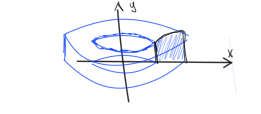
\includegraphics[width = 10 cm]{assets/integral-v-figure.png}
\end{center}

$a>0,b>0, f>0$. Вращаем ПГ$(f[a,b])$ вокруг оси $Oy$. Получается вот что-то такое(см рисунок). Хочу найти объем этой фигуры 

$\varPhi([a,b]) = Vol(\{(x,y,z): a^2\leq x^2 + y^2 \leq b^2, 0\leq z \leq f(\sqrt{x^2+y^2})\})$. Тогда выполнено:
$$\varPhi([a,b]) = 2\pi \integral{a}{b}xf(x)dx$$

\subsection{Вычисление длины гладкого пути}

$\sigma (\text{ПГ($f, [a,b]$)}) = \integral{a}{b}f\, dx$, где $f \geq 0, f$ - непрерывно.
$\gamma(t) =  \left (\begin{gathered}
    x = x(t)\\
    y(x) = y(t)
\end{gathered}\right)$, $\gamma:[p,q] \rightarrow R^2$.
\begin{center}
   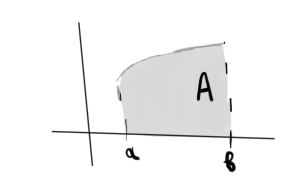
\includegraphics[width = 7 cm]{assets/integral_4.png}
\end{center}
\textbf{Замечание от Славы}: вообще $x(t)$ должно монотонно возрастать, иначе странные загагулины будут давать одну и ту же площадь, но КПК про это ничего не сказал.

Причем $\gamma$ -  гладкое изоображение (дифференцируема столько раз сколько надо).

Получилась какая-то кривая (как на рисуночке сверху), и я хочу смотреть подграфики такой кривой. Тогда:
$$\sigma A = \integral{a}{b}"y(x)"dx = \left[\begin{gathered}
    x = x(t)\\
    y = y(t)
\end{gathered}\right] = \integral{p}{q}y(t) x'(t) dt$$
Теперь мы умеем вычислять интегралы не только в декартовых координатах.


\subsection{Свойства верхнего и нижнего пределов}

\thmm{Теорема (о свойствах верхнего и нижнего предела)}

$(x_n), (\overline{x_n})$ --- произвольные вещ последовательности

\begin{enumerate}
    \item $\underline{\lim}x_n \leq \overline{\lim }x_n$
    \item Если $\forall n : x_n \leq \overline{x_n}$, то $\overline{\lim} x_n\leq \overline{\lim} \overline{x_n}$ и $\underline{\lim} x_n\leq \underline{\lim} \overline{x_n}$
    
    \textbf{Замечание от Славы:} На самом деле здесь можно сказать, что $\exists N$ начиная с которого выполнено $x_n \leq \overline{x_n}$, но КПК почему-то решил так ввести это свойство.

    \item $\forall \lambda \in\mathbb{R}, \lambda\geq 0$. Тогда $\overline{\lim}\lambda x_n = \lambda \overline{\lim} x_n$ и $\underline{\lim}\lambda x_n = \lambda \underline{\lim} x_n$. (Считаем $0 \cdot \infty = 0$)
    \item $\overline{\lim}(-x_n)= - \underline{\lim}x_n$
    \item $\overline{\lim }(x_n + \overline{x}_n) \leq \overline{\lim }  {x}_n + \overline{\lim }\overline{x}_n $
    \item Пусть $t_n \rightarrow l \in \R$. Тогда $\overline{\lim}(x_n + t_n) = \overline{\lim} (x_n) + l $ и $\underline{\lim}(x_n + t_n) = \underline{\lim} (x_n) + l $
    \item $t_m \rightarrow l>0 (l\in \R)$. Тогда $\overline{\lim} (t_nx_n) =l  \overline{\lim} (x_n)$ и  $\underline{\lim} (t_nx_n) =l  \underline{\lim} (x_n)$
\end{enumerate}

\subsection{Техническое описание верхнего предела}


\thmm{Теорема (техническое определение верхнего предела).}

$(x_n)$ - произвольная вещ. последовательность.

\begin{enumerate}
    \item $\overline{\lim}x_n = + \infty \Leftrightarrow x_n$ - не ограничено сверху
    \item $\overline{\lim}x_n = - \infty \Leftrightarrow x_n \rightarrow - \infty$.
    \item $\overline{\lim}x_n = l \Leftrightarrow$
    \begin{enumerate}
        \item $\forall \varepsilon >0: \exists :\forall n>N: x_n<l+\varepsilon$
        \item $\forall \varepsilon >0$ неравенство $l-\varepsilon\leq x_n$ выполнено для бесконечного множества $x$-ов
    \end{enumerate}
\end{enumerate}

\subsection{Теорема о существовании предела в терминах верхнего и нижнего пределов}

\thmm{Теорема}

$\exists \lim(x_n) = L \in \overline{\mathbb{R}} \Leftrightarrow \underline{\lim}x_n = \overline{\lim} x_n = L$.


\subsection{Теорема о характеризации верхнего предела как частичного}

$(x_n)$ - вещ последовательность. Тогда:

\begin{enumerate}
    \item Если $l \in \overline{\mathbb{R}} - $ частичный предел $x_m$, то $\underline{\lim}x_n\leq l \leq \overline{\lim}x_n$
    \item $\exists n_k, m_k: x_{n_k}\rightarrow \overline{\lim} x_{n}, x_{m_k}\rightarrow \underline{\lim}x_n$
\end{enumerate}

\subsection{Интеграл как предел интегральных сумм}

\thmm{Теорема(об интеграле, как о пределе частичных сумм)}

$f\in C([a,b])$. Тогда $\forall \varepsilon >0: \exists \delta >0 : \forall$ дробления $(x_0,\ldots,x_m)$ ранга $< \delta$. Тогда $\forall$ оснащ.:
$$\left|\integral{a}{b}f(x)dx - \sum\limits_{i=1}^nf(\xi_i) (x_i-x_{i-1})\right|<\varepsilon$$

\subsection{Теорема об интегральных суммах центральных прямоугольников и трапеций}

\thmm{Теорема (об интегральной сумме центральных прямоугольников)}

$f \in C^2([a,b])$, $a = x_0<x_1<\ldots< x_n =b$, $\delta = max(x_i-x_{i-1}), \xi_i = \cfrac{(x_{i-1}+x_i)}{2}$.

Тогда:
$$\left|\sum\limits_{i=1}^m f(\xi_i)(x_i-x_{i-1}) - \integral{a}{b}f(x) dx\right|\leq \cfrac{\delta^2}{8}\integral{a}{b} |f''(x)|dx$$
\thmm{Теорема (формула трапеций)}

в тех же условиях:
$$\left|\sum\limits_{i=1}^n (\cfrac{f(x_i)+f(x_{i-1})}{2}(x_i-x_{i-1}))-\integral{a}{b}f(x) dx\right|\leq \cfrac{\delta^2}{8}\integral{a}{b} |f''(x)|dx$$

\subsection{Формула Эйлера--Маклорена. Асимптотика степенных сумм}

\thmm{Формула Эйлера - Маклорена (простейшая)}

$f \in C^2([m,n])$, $m,n \in \mathbb{R}$. Тогда:

$\sum\limits_{i=m}^n f(i) - \cfrac{1}{2}f(m) - \cfrac{1}{2}f(n)= \integral{m}{n}{f(x)}{dx}+ \cfrac{1}{2}\integral{m}{n}f''(x)\{x\}(1-\{x\})dx$

\subsection{Асимптотика частичных сумм гармонического ряда}

$f(x) = x^p$ $(p> -1)$
$$1^p+2^p+\ldots + n^p= \integral{1}{n}x^pdx + \cfrac{1}{2}(n^p+1)+\cfrac{1}{2}\integral{1}{n}p(p-1)x^{p-2}\{x\}(1-\{x\}) =$$$$= \cfrac{n^{p+1}}{p+1}-\cfrac{1}{p+1}+\cfrac{n^p}{2}+\cfrac{1}{2} + O(\max(1,n^{p-1}) = \cfrac{n^{p+!}}{p+1} + \cfrac{n^p}{2} + O(max(1,n^{p-1}))$$
Торжественный момент, применим формулу для $p=1$:

$1 + 2 + \ldots + n = \cfrac{n^2}{2}+\cfrac{n}{2}+0$ --- Мы доказали теорему Гаусса.

Применим формулу для $p=-1$:

$1+ \cfrac{1}{2}+ \cfrac{1}{3}+ \ldots + \cfrac{1}{n} = \ln n + \cfrac{1}{2} + \cfrac{1}{2n}+\integral{1}{n}\cfrac{1}{x^3}\{x\}(1-\{x\})dx$

$1+\cfrac{1}{2}+\cfrac{1}{3}+\ldots +\cfrac{1}{n}= \ln n + \gamma + o(1)$. Причем $\gamma \in [\cfrac{1}{2},\cfrac{5}{8}]$ - \deff{Постоянная Эйлера}

\subsection{Формула Валлиса}

\deff{Формула Валлиса}

$I_n = \integral{0}{\frac{\pi}{2}}\sin^nxdx = \begin{cases}
    \cfrac{(n-1)!!}{n!!}\cfrac{\pi}{2}, n - \text{четная}\\
    \cfrac{(n-1)!!}{n!!}, n - \text{неч}
\end{cases}$

КПК: Используйте формулу интегрирования по частям. Двойной факториал - одной четности

$x\in [0,\frac{\pi}{2}]$

$\sin^{2k+1} x\leq \sin^{2k}x\leq \sin^{2k-1}x$ - очевидное неравенство. Проинтегрируем по $0,\cfrac{\pi}{2}$, получим:
$$\cfrac{(2k)!!}{(2k+1)!!}\leq \cfrac{(2k-1)!!}{2k!!}\cdot \cfrac{\pi}{2}\leq \cfrac{(2k-2)!!}{(2k-1)!!}$$
$$\left(\cfrac{(2k)!!}{(2k-1)!!}\right)^2\cfrac{1}{2k+1} \leq \cfrac{\pi}{2}\leq \left(\cfrac{(2k)!!}{(2k-1)!!}\right)^2\cfrac{1}{2k}$$
Правая часть - левая часть $\left(\cfrac{(2k)!!}{(2k-1)!!}\right)^2(\cfrac{1}{2k}\cdot\cfrac{1}{2k+1})\leq \cfrac{\pi}{2}\cdot \cfrac{1}{2k} \rightarrow 0$

Получили, что левая и правые величины стремятся к $\frac{\pi}{2}$.

$\lim\limits_{k\rightarrow\infty}\left(\cfrac{(2k)!!}{(2k-1)!!}\right)^2\cfrac{1}{k} = \pi$ --- \deff{Формула Валлиса}

\subsection{Формула Стирлинга.}
\thmm{Формула Стирлинга}

Воспользуемся формулой Эйлера - Маклорена для $f(x) = \ln x$:
$$\ln 1 + \ln 2 + \ldots + \ln n = \integral{1}{n}\ln x dx +\cfrac{\ln n }{2} - \cfrac{1}{2}\integral{1}{n}\cfrac{1}{x^2}\{x\}(1-\{x\})dx = $$
$$n\ln n - n + 1 +\cfrac{\ln n}{2} - \cfrac{1}{2}\integral{1}{n}\cfrac{1}{x^2}\{x\}(1-\{x\})dx = n \ln n - n +\cfrac{\ln 2}{2} +C_1 + o(1)$$
А давайте теперь возвем экспоненту от правой и левой части:
$$n! = e^{n\ln n}e^{-n}e^\frac{\ln n}{2} e^{C_i + o(1)}$$
Получили, что $n!\, \mytilde\, \cfrac{n^n}{e^n}\sqrt{n}\cdot c$, где $c = e^{C_1}$.

А теперь давайте сочетать и найдем эту $c$.

$(2k)!! = k!\cdot 2^k, (2k-1)!! = \cfrac{(2k)!}{k!\cdot2^k}$. С учетом этого воспользуемся формулой Валлиса:
$$\sqrt{\pi} = \lim\limits_{k\rightarrow\infty}\left(\cfrac{(2k)!!}{(2k-1)!!}\right)\cfrac{1}{\sqrt{k}}=\lim_{k\rightarrow \infty}\cfrac{2^{2k}(k!)^2}{(2k)!}\cfrac{1}{\sqrt{k}} = \lim_{k\rightarrow \infty} \cfrac{2^{2k}k^{2k}e^{-2k}k\cdot c^2}{(2k)^{2k}e^{-2k}\sqrt{2k}\cdot c}\cfrac{1}{\sqrt{k}} = \cfrac{c}{\sqrt{2}}$$
Откуда $c = \sqrt{2\pi}$

$n!\, \mytilde\, \cfrac{n^n}{e^n}\sqrt{n}\cdot \sqrt{2\pi}$ --- \deff{Формула Стирлинга}
\subsection{Простейшие свойства несобственного интеграла}

\textbf{Свойства:}
\begin{enumerate}
    \item \textbf{Критерий Больцана-Коши} (сходимости несобственного интеграла):
  
  $\integral{a}{b}f(x)dx$ --- сходящаяся $\Leftrightarrow \forall \varepsilon >0:\exists \Delta \in (a,b): \forall A,B\in \Delta,  |\integral{A}{B}f|< \varepsilon$
  

  \textbf{Следствие:} Если $\exists A_n,B_n \rightarrow b-0: \integral{A_n}{B_n}f \not \rightarrow 0$, то $\integral{a}{b}f$ - расходится.

  \item Аддитивность на промежутке:

$f$ - допустима на $[a,b)$, $c \in (a,b)$. Тогда $\integral{a}{c}, \integral{c}{b}$ сходятся или расходятся одновременно и в случаях сходимости $\integral{a}{b}f = \integral{a}{c}f + \integral{c}{b}f$

Если $\integral{a}{b}f$ сходится, то $\integral{c}{b} f \rightarrow 0$, при $c\rightarrow b - 0$.

\item $f,g$ - доп на $[a.b)$, $\integral{a}{b}f,\integral{a}{b}g$ - сходятся, $\lambda\in \mathbb{R}:$

Тогда $\integral{a}{b}f +g = \integral{a}{b}f + \integral{a}{b}g, \integral{a}{b}\lambda f = \lambda \integral{a}{b}f$

\item  $f,g$ допустимы на $[a,b)$: $\integral{a}{b}g,\integral{a}{b}f$ - существует в $\mathbb{R}$, $f\leq g$. Тогда $\integral{a}{b}f \leq \integral{a}{b}g$.

\item $f,g$ - дифф. на $[a,b)$, $f',g'$ - допустимы, тогда:
$$\integral{a}{b}fg' = fg\Big|_a^b - \integral{a}{b}f'g$$
(если существуют два предела из трех)

\item $\varphi: [\alpha, \beta) \rightarrow \langle A, B \rangle, \varphi \in C.$ Пусть $\exists \varphi(\beta-0)\in \overline{\mathbb{R}}, f\in C(\langle A,B\rangle)$. Тогда:
$$\integral{\alpha}{\beta}f(\varphi)\varphi'dt = \integral{\varphi(\alpha)}{\varphi(b-0)}f(x) dx$$

\end{enumerate}


\subsection{Признаки сравнения сходимости несобственного интеграла}

\thmm{Лемма:}

Пусть $f$ допустима на $[a,b), f\geq 0, \varPhi(A) = \integral{a}{A}f$.  Тогда $\integral{a}{b}$ - сходящаяся, то $\varPhi$ ограниченная.


\textbf{Признак сравнения.}

$g \geq 0 ,f \geq 0$ допустимы на $[a,b)$

\begin{enumerate}
    \item $f\leq g$, если $g$ сходится, то $f$ очевидно сходится и если $f$ расходится, то $g$ тоже расходится.
    \item $\lim\limits_{x\rightarrow b-0} \cfrac{f(x)}{g(x)} = e\in (0, +\infty)$, то $\integral{a}{b}f,\integral{a}{b}g$ сходятся и расходятся одновременно.
    \item $\lim\limits_{x\rightarrow b-0}\cfrac{f(x)}{g(x)}=0$, то выполнен пункт 1, если предел бесконечность, то поменяйте $f,g$ местами.
\end{enumerate}

\subsection{Изучение сходимости интеграла $\int_{10}^\infty \frac{dx}{x^\alpha (\ln x)^\beta}$}

не думаю, что это будет

\subsection{Гамма функция Эйлера. Простейшие свойства. Интеграл Эйлера--Пуассона}

\deff{Гамма функция Эйлера} --- $\Gamma(t) = \integral{0}{+\infty}x^{t-1}e^{-x} dx, t \in (0,+\infty)$

1) При $t>0$ интеграл сходится. 

2) $\Gamma(t)$ непрерывна, потому что $\Gamma(t)$ - выпуклая функция. А почему она выпуклая? Посмотрим на функцию $t\rightarrow x^{t-1}e^{-x}$. Вторая производная (по $t$) больше нуля, откуда она выпуклая. Тогда и $\Gamma(t)$ выпуклая, а отсюда непрерывная. Мы просто пишем неравенство выпуклой функции и интегрируем его.

3) $\forall t >0: \Gamma(t+1) = t \Gamma(t)$, в частности $\Gamma(n+1) = n (n-1) \ldots 1 = n!$

$\Gamma(t+1) = \integral{0}{+\infty}x^t e^{-x} dx = x^t (-e^{-x})\Big|^{+\infty}_{0} + t \integral{0}{+\infty}x^{t-1}e^{-x} dx= t\Gamma(T)$

4) $t \Gamma(t) \mytilde 1$, $\Gamma(t) \mytilde \cfrac{1}{t}$ при $t\rightarrow 0 $

5) $\Gamma(\cfrac{1}{2}) = \sqrt{\pi}$ - \deff{Интеграл Эйлера - Пуассона}. $\integral{0}{+\infty}e^{-x^2}dx = \cfrac{1}{2}\sqrt{\pi}$ --- точнее вот он.

\subsection{Теорема об абсолютно сходящихся интегралах и рядах.}

\thmm{Теорема.}

$f$ - допустима на $[a,b)$. Тогда эквивалетно:

\begin{enumerate}
    \item $\integral{a}{b}f$ - абсолютно сходится.
    \item $\integral{a}{b}|f|$ - сходится
    \item $\integral{a}{b} f^+, \integral{a}{b} f^{-}$ - оба сходятся.
\end{enumerate}


\thmm{Теорема.}

$a_n$ --- любого знака. Тогда эквивалентно:
\begin{enumerate}
    \item $\sum\limits_{}a_n$ - абсолютная сходимость.
    \item $\sum\limits_{}|a_n|$ - сходится.
    \item $\sum a_n^+, \sum a_n^-$ - оба сходятся. Где $a_n^+ = \max(a_n,0), a^-_n= \max(-a_n,0)$
\end{enumerate}

\subsection{Изучение интеграла $\int_1^{\infty} \frac{\sin x\,dx}{x^p}$ на сходимость и абсолютную сходимость}

не думаю, что это будет

\subsection{Признак Абеля--Дирихле сходимости несобственного интеграла}

\thmm{Теорема (Признак Абеля-Дирихле)}

\begin{enumerate}
    \item $f$ - допустима на $[a,b)$. $F(A) = \integral{a}{A}f(x)dx$ - ограничена на $[a,b)$. $\exists k: \forall A \in [a,b): |\integral{a}{A}f(x)|\leq K$
    
    Пусть есть $g\in C^1([a,b))$, $g$ - монотонна и $g(x)\rightarrow 0$ при $x\rightarrow b$. Тогда $\integral{a}{b} f(x) g(x)dx$ - сходится.
    \item $f$ - допустима на $[a,b)$, $\integral{a}{b}f(x)dx$ - сходится. $g \in C^1([a,b))$, $g$ - монотонна и ограничена на $[a,b)$. Тогда $\integral{a}{b} f(x) g(x)dx$ - сходится.
\end{enumerate}

\subsection{Интеграл Дирихле.}

\textbf{Пример (Интеграл Дирихле)}

$\integral{0}{+\infty}\cfrac{\sin x}{x}dx  =\cfrac{\pi}{2}$

\subsection{Свойства рядов: линейность, свойства остатка, необх. условие сходимости, критерий Больцано--Коши}

\textbf{Свойства рядов:}

\begin{enumerate}
    \item $\sum a_n , \sum b_n$ - сх. $c_n = a_n + b_n$.

        Тогда $\sum c_n$ - сходится и $\sum c_n = \sum a_n + \sum b_n$
    \item $\sum a_n$  - сходится $\lambda\in \mathbb{R} \Rightarrow \sum\lambda a_n$ - сходится и $\sum \lambda a_n = \lambda \sum a_n$.
    \item $\sum a_n$ - сходится, то любой остаток ряда сходится
    \item Если какой-нибудь остаток ряда сходится, то ряд сходится
    \item Ряд сходится $\Leftrightarrow r_n \rightarrow 0 $.
\end{enumerate}

\thmm{Теорема (грабли) (необходимое условие сходимости)}

$\sum a_n$ - сходится. Тогда $a_n \rightarrow 0$


\textbf{Замечание.} В ОБРАТНУЮ СТОРОНУ НЕ РАБОТАЕТ!!!

\thmm{Теорема (критерий Больцано-Коши)}

$\sum a_n$ - сходится $\Leftrightarrow \forall \varepsilon>0: \exists N:\forall n > N: \forall k \in \mathbb{N}: |\sum\limits_{i=n+1}^{n+k}a_n|<\varepsilon$

\subsection{Признак сравнения сходимости положительных рядов}

\thmm{Теорема (Признак сравнения)}

Есть $a_k \geq 0 , b_k \geq 0$

\begin{enumerate}
    \item  $\forall n: a_n \leq b_n$. Тогда, если $b$ сходится $\Rightarrow$  $a$ сходится. Если $a$ расходится, то $b$ расходится.
    \item $\cfrac{a_n}{b_n}\rightarrow l$. Если $ l \in (0,+\infty)$, тогда a,b сходятся расходятся одновременно. Если $l = 0$, то выполнено утв. из пункта 1. Если $l=+\infty$, то выполнено утв. из пункта 1 наоборот
    \item Начиная с некоторого места $\cfrac{a_{n+1}}{a_n}\leq \cfrac{b_{n+1}}{b_n}$, то см утв. пункт 1.
\end{enumerate}

\subsection{Признак Коши сходимости положительных рядов}

\thmm{Теорема (Признак Коши)}

$\sum a_n, a_n \geq 0 , K_n = \sqrt[n]{a_n}$

light:
\begin{enumerate}
    \item $\exists q \in (0,1)$, $K_n \leq q$. Тогда $\sum a_n$ - сходится
    \item $K_{n}\geq 1$ для бесконечного множества номеров. Тогда $\sum a_n$ - расходится
\end{enumerate}
pro:

$K = \overline{\lim} K_n$
\begin{enumerate}
    \item $K>1$ ряд расходится.
    \item $K<1$ ряд сходится
\end{enumerate}

\textbf{Замечание} $K=1$ - признак не работает.

\subsection{Признак Даламбера сходимости положительных рядов}

\thmm{Теорема (Признак Даламбера)}

$a_n > 0: D_n = \cfrac{a_{n+1}}{a_n}$

light: 
\begin{enumerate}
    \item $\exists q \in (0,1): D_n \leq q$ НСНМ. Тогда $\sum a_n$ - сходится
    \item $D_n \geq 1$ НСНМ. Тогда $\sum a_n$ - расходится.
\end{enumerate}

pro: $D:= \lim D_n$
\begin{enumerate}
    \item $D>1$: Ряд расходится
    \item $D<1$: Ряд сходится
\end{enumerate}

\subsection{Признак Раабе сходимости положительных рядов}

\thmm{Признак (Раабе)}

$a_n > 0$. $R_n := n(\cfrac{a_n}{a_{n+1}}-1)$

light:
\begin{enumerate}
    \item $\exists r>1:$ НСНМ $R_n \geq r \Rightarrow $ Ряд $\sum a_n$ сходится
    \item $R_n\leq 1$ НСНМ $\Rightarrow$ Ряд $\sum a_n$ расходится
\end{enumerate}
pro:

$R:= \lim R^n$
\begin{enumerate}
    \item $R>1$: ряд сходится
    \item $R<1$: расходится.
\end{enumerate}

\subsection{Интегральный признак Коши сходимости числовых рядов}

\thmm{Теорема (Интегральный признак Коши)}

Пусть у вас есть функция $f$ - непрерывная на $[1,+\infty)$, монотонна, $f\geq 0 $. Тогда $\sum\limits_{n=1}^{+\infty}f(n)$ и $\integral{1}{+\infty}f(x)dx$ сходятся и расходятся одновременно.

\subsection{Признак Лейбница}

\thmm{{Теорема (Признак Лейбница)}}

$c_1 \geq c_2 \geq \ldots \geq 0$ (т.е монотонность). Пусть $c_n \rightarrow 0 $. Тогда $\sum\limits_{n=1}^{+\infty} (-1)^{n+1} c_n$ - сходится.

\subsection{Признаки Дирихле и Абеля сходимости числового ряда}


\thmm{Теорема (признак Абеля и Дирихле)}

\begin{enumerate}
    \item
    \begin{enumerate}
        \item  Пусть частичные суммы последовательности $a_n$ - ограниченны: $\exists C_A: \forall n: a_1 + \ldots + a_n \leq C_A$.
         \item Пусть $b_n$ - монотонна, $b_n\rightarrow 0 $
    
    \end{enumerate}
     Тогда $\sum\limits_{n=1}^{+\infty}a_nb_n$ - сходится
  
   \item
   \begin{enumerate}
       \item Ряд $\sum a_n$ - сходится.
        \item $b_n$ - монотонна и ограничена. $\exists C_B: \forall $
   \end{enumerate}
    Тогда $\sum\limits_{n=1}^{+\infty}a_nb_n$ - сходится.
   
\end{enumerate}

\end{document}


